\documentclass[titlepage,a4paper]{article}

\usepackage{a4wide}
\usepackage[colorlinks=true,linkcolor=black,urlcolor=blue,bookmarksopen=true]{hyperref}
\usepackage{bookmark}
\usepackage{fancyhdr}
\usepackage[spanish]{babel}
\usepackage[utf8]{inputenc}
\usepackage[T1]{fontenc}
\usepackage{graphicx}
\usepackage{float}
\usepackage[left=2.5cm, top=2.5cm, right=2.5cm, bottom=2.5cm]{geometry}
\usepackage{listings}
\usepackage{xcolor}

\definecolor{codegreen}{rgb}{0,0.6,0}
\definecolor{codegray}{rgb}{0.5,0.5,0.5}
\definecolor{codepurple}{rgb}{0.58,0,0.82}
\definecolor{backcolour}{rgb}{0.95,0.95,0.92}

\lstdefinestyle{mystyle}{
    backgroundcolor=\color{backcolour},   
    commentstyle=\color{codegreen},
    keywordstyle=\color{magenta},
    numberstyle=\tiny\color{codegray},
    stringstyle=\color{codepurple},
    basicstyle=\ttfamily\footnotesize,
    breakatwhitespace=false,         
    breaklines=true,                 
    captionpos=b,                    
    keepspaces=true,                 
    numbers=left,                    
    numbersep=5pt,                  
    showspaces=false,                
    showstringspaces=false,
    showtabs=false,                  
    tabsize=2
}

\lstset{style=mystyle}


\usepackage{underscore} % Permite usar el carácter _ como literal

\pagestyle{fancy} % Encabezado y pie de página
\fancyhf{}
\fancyhead[L]{TP1 - File Transfer}
\fancyhead[R]{Redes- FIUBA}
\renewcommand{\headrulewidth}{0.4pt}
\fancyfoot[C]{\thepage}
\renewcommand{\footrulewidth}{0.4pt}

\begin{document}
\begin{titlepage} % Carátula
    \hfill
\includegraphics[width=6cm]{img/logofiuba.jpg}
    \centering
    \vfill
    \Huge \textbf{Trabajo Práctico 2 —  Software-Defined Networks}
    \vskip2cm
    \Large [TA048] Redes \\
    Curso 2 \\ 
    \vfill
    \begin{tabular}{ | l | l | l |}
      \hline
      Alumno & Número de padrón & Email \\ \hline
      Lucas Oshiro & 107024 & loshiro@fi.uba.ar \\ \hline
      Martin Reimundo & 106716 & mreimundo@fi.uba.ar \\ \hline
      Franco Agustin Rodriguez & 108799 & frodriguez@fi.uba.ar \\ \hline
      Mateo Riat Sapulia & 106031 & mriat@fi.uba.ar \\ \hline
      Ignacio Vetrano & 106129 & ivetrano@fi.uba.ar \\ \hline
    \end{tabular}
    \vfill
    \vfill
\end{titlepage}

\tableofcontents % Índice general
\newpage

\section{Introducción}\label{sec:intro}

    Este trabajo práctico tiene como objetivo introducir los conceptos fundamentales detrás de SDN y OpenFlow, y familiarizarse con la programación de dispositivos de red a través de una API. Se buscará comprender cómo estos enfoques permiten un control más preciso sobre el funcionamiento de los switches y habilitan una infraestructura de red más ágil, adaptable y preparada para las necesidades de hoy en día.



\section{Hipótesis y supuestos realizados}\label{sec:supuestos}

    \begin{itemize}
        \item La topología cuenta con al menos un switch. \\

        \item El firewall está configurado en un único switch, por lo que las reglas se aplicarán únicamente si el tráfico entre el host origen y el host destino pasa a través de dicho switch.
    \end{itemize}
    
\section{Implementación}\label{sec:implementacion}
A continuación se mostrará la implementación realizada. Se realizaron dos implementaciones, una para la topologia y otra para el firewall.

\subsection{Topologia}
\lstinputlisting[language=Python]{src/topology.py}
\\

\subsubsection{Implementación}
\begin{itemize}
    \item Nuestra topologia recibe por parametro la cantidad de switches que se necesitan. \item Creamos 4 host especificandoles sus MAC address.
    \item Luego creamos la cantidad de switches correspondientes.
    \item Creamos la conexión con el primer switch y los hosts 1 y 2.
    \item Conectamos todos los switches y al último switch le añadimos las conexiones con los hosts 3 y 4.
\end{itemize} 

\subsection{Firewall}
\lstinputlisting[language=Python]{src/firewall.py}

\section{Pruebas}\label{sec:pruebas}

En esta sección se mostrarán las pruebas realizadas.

\subsection{Regla 1: No se aceptan mensajes al puerto 80}
Se intentará enviar un mensaje desde el host 1 al host 4 al puerto 80 utilizando TCP.

\begin{figure}[H]
    \centering
    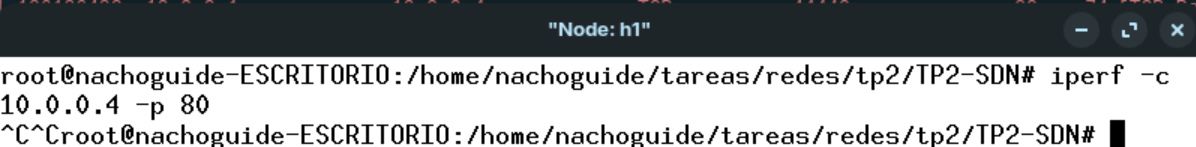
\includegraphics[width=0.7\textwidth]{img/regla1_h1_tcp.png}
    \caption{Regla 1 desde el host 1 (TCP)}
\end{figure}

\begin{figure}[H]
    \centering
    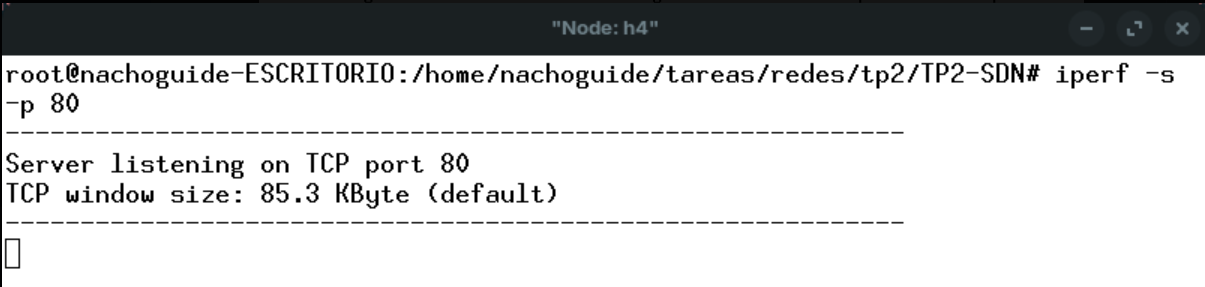
\includegraphics[width=0.7\textwidth]{img/regla1_h4_tcp.png}
    \caption{Regla 1 desde el host 4 (TCP)}
\end{figure}

\begin{figure}[H]
    \centering
    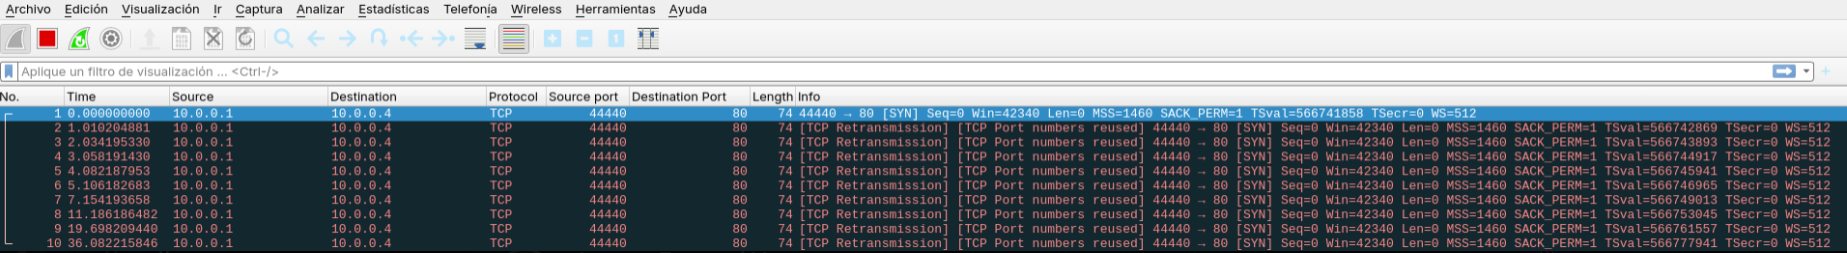
\includegraphics[width=0.7\textwidth]{img/regla1_wireshark_tcp.png}
    \caption{Wireshark para la regla 1 (TCP)}
\end{figure}

Se observa como desde h1 envia un mensaje SYN, pero desde el h4 no recibe respuesta. A su vez, desde el host 4 no envia ni recibe mensajes al host 1.

También realizamos la prueba usando UDP.

\begin{figure}[H]
    \centering
    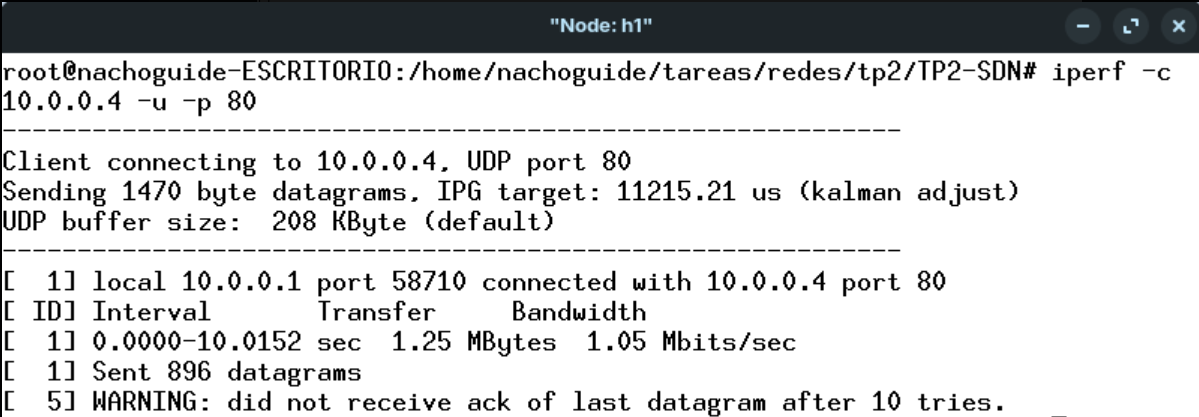
\includegraphics[width=0.7\textwidth]{img/regla1_h1_udp.png}
    \caption{Regla 1 desde el host 1 (UDP)}
\end{figure}

\begin{figure}[H]
    \centering
    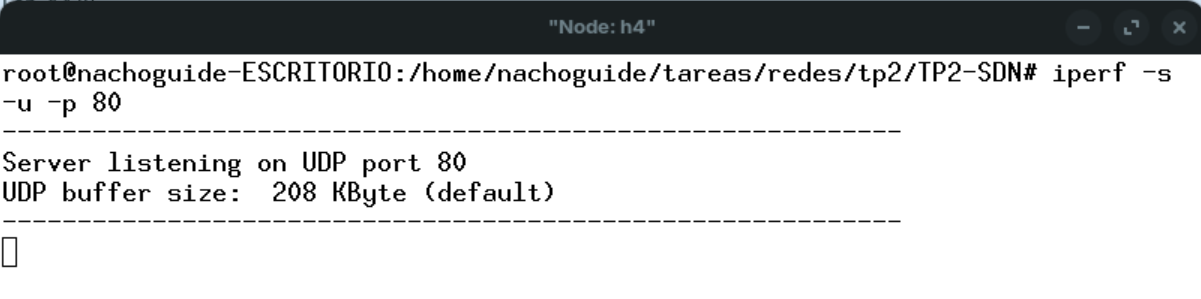
\includegraphics[width=0.7\textwidth]{img/regla1_h4_udp.png}
    \caption{Regla 1 desde el host 4 (UDP)}
\end{figure}

\begin{figure}[H]
    \centering
    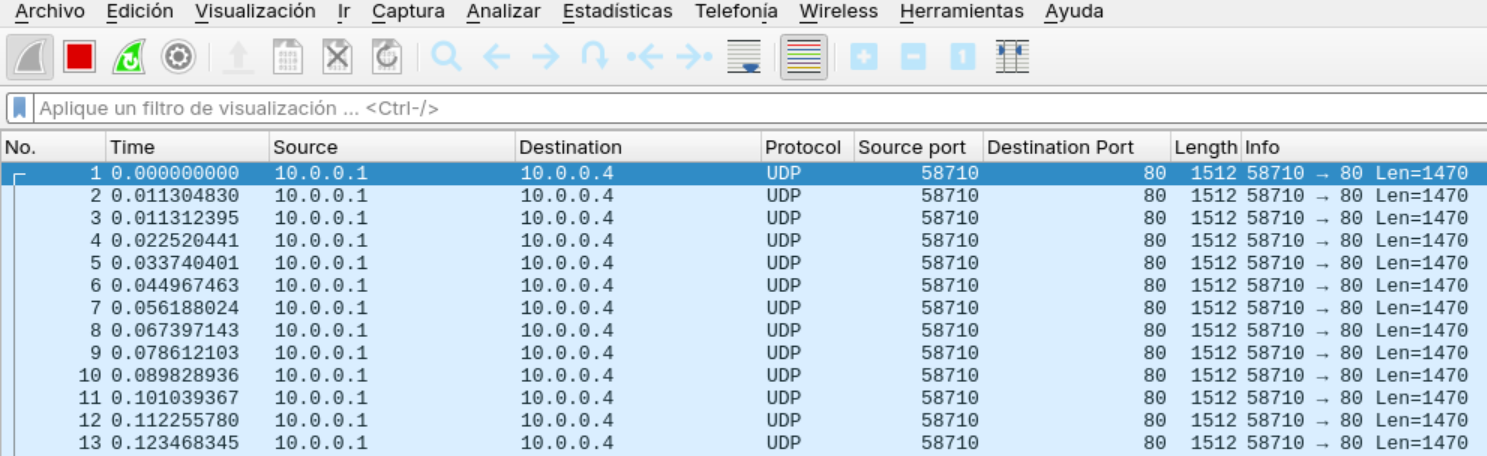
\includegraphics[width=0.7\textwidth]{img/regla1_wireshark_udp.png}
    \caption{Wireshark para la regla 1 (UDP)}
\end{figure}

Se observa como desde el host 1 se envian los mensajes, pero no recibe ningún ack por parte del host 4.
Desde la perspectiva del host 4, no se envian ni se reciben mensajes al host 1.



\subsection{Regla 2: Se descartan los mensajes del host 1 con puerto de destino 50001, usando UDP}
En esta prueba, se descartan todos los mensajes provenientes del host 1 con puerto destino 5001 y que se este usando UDP.

\begin{figure}[H]
    \centering
    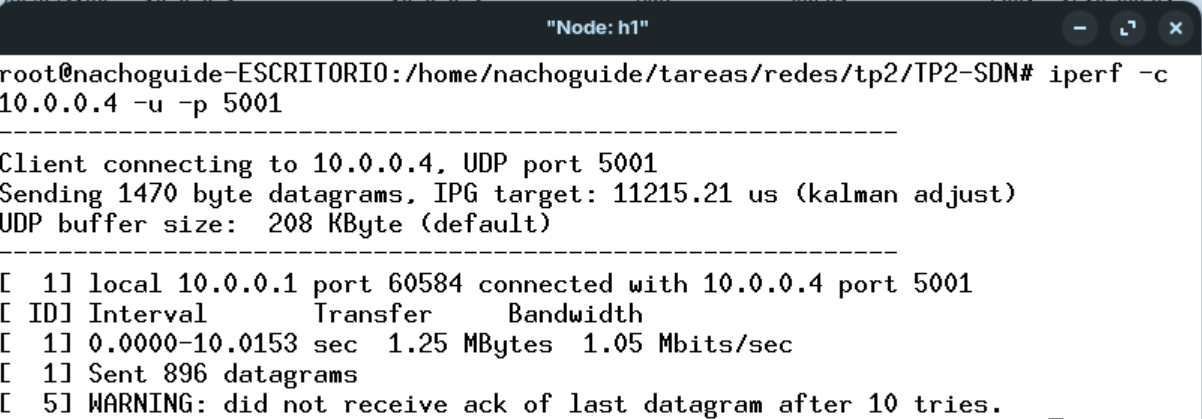
\includegraphics[width=0.7\textwidth]{img/regla2_h1_udp.png}
    \caption{Regla 2 desde el host 1 (UDP)}
\end{figure}

\begin{figure}[H]
    \centering
    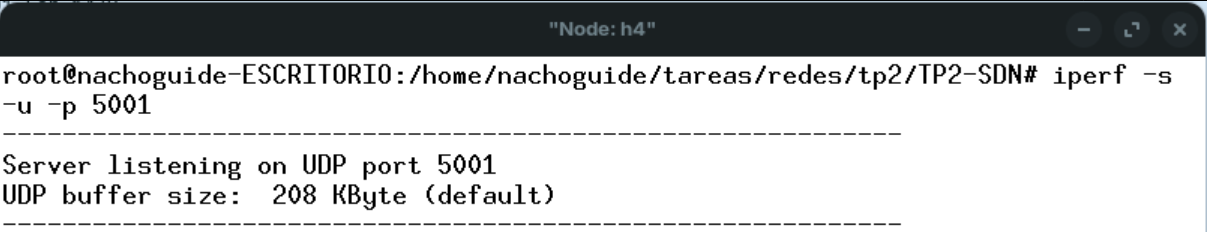
\includegraphics[width=0.7\textwidth]{img/regla2_h4_udp.png}
    \caption{Regla 2 desde el host 4 (UDP)}
\end{figure}

\begin{figure}[H]
    \centering
    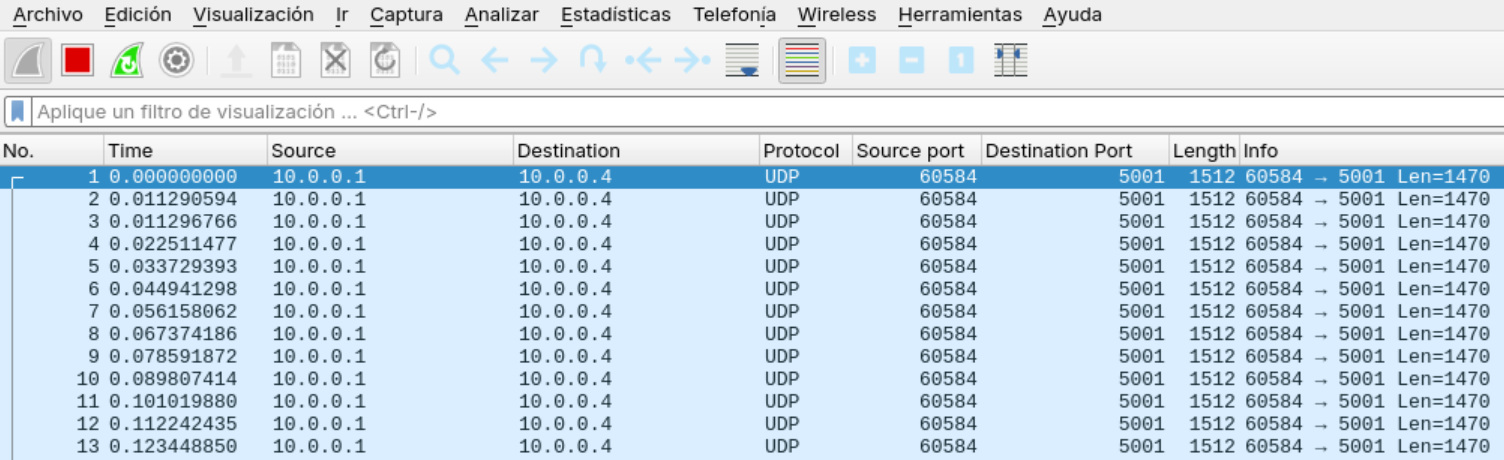
\includegraphics[width=0.7\textwidth]{img/regla2_wireshark_udp.png}
    \caption{Wireshark para la regla 2 (UDP)}
\end{figure}

Podemos observar, que desde el host 1 se envian los mensajes al puerto 5001 del host 4, pero no llegan ningún ack como respuesta por parte del host 4.
Desde el lado del host 4, no se realiza ninguna acción.

Probaremos enviar mensajes usando TCP y a otro puerto

\begin{figure}[H]
    \centering
    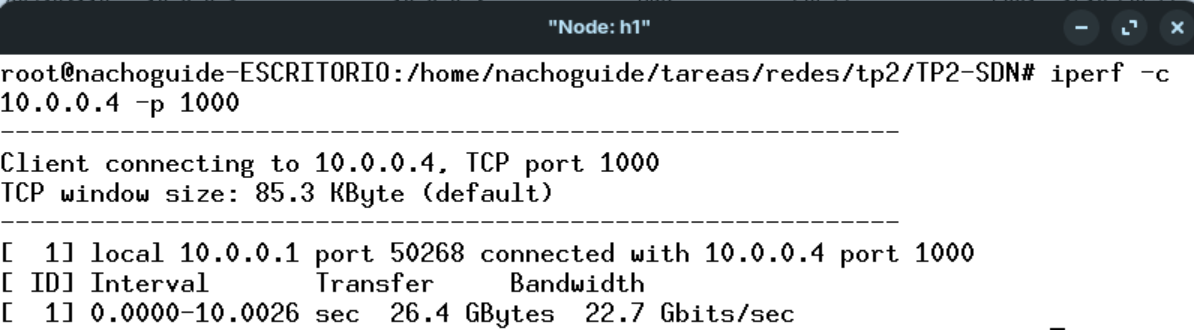
\includegraphics[width=0.7\textwidth]{img/regla2_h1_tcp.png}
    \caption{Regla 2 desde el host 1 (TCP)}
\end{figure}

\begin{figure}[H]
    \centering
    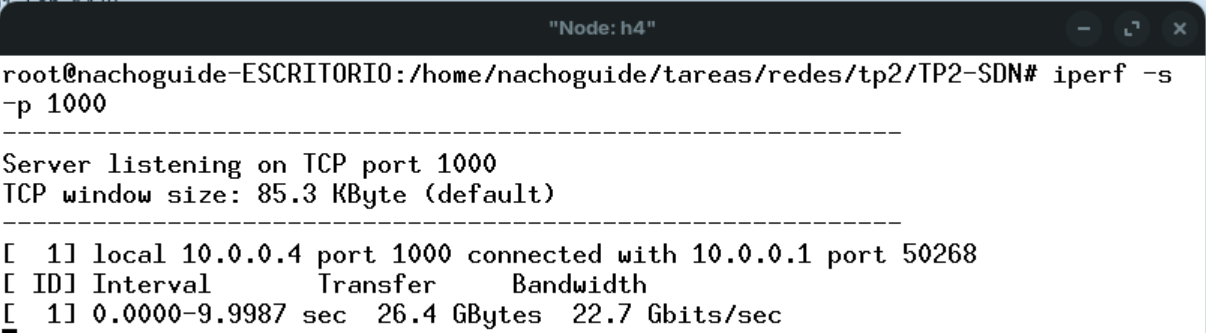
\includegraphics[width=0.7\textwidth]{img/regla2_h4_tcp.png}
    \caption{Regla 2 desde el host 4 (TCP)}
\end{figure}

\begin{figure}[H]
    \centering
    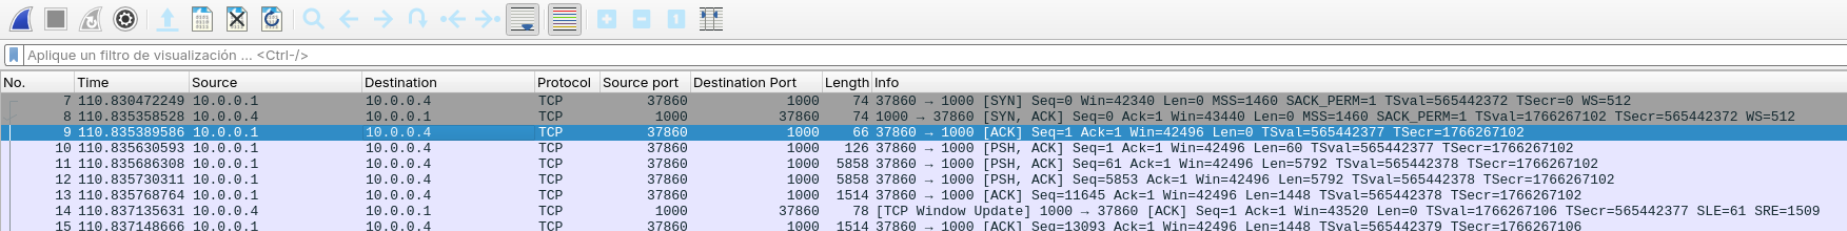
\includegraphics[width=0.7\textwidth]{img/regla2_wireshark_tcp.png}
    \caption{Wireshark para la regla 2 (TCP)}
\end{figure}

En este caso, al utilizar TCP y enviar los mensajes al puerto 1000, se observa que el host 1 envió mensajes y recibió respuestas por parte del host 4.

\subsection{Regla 3: No se pueden conectar el host 1 y el host 3}
Ahora probamos enviar mensajes desde el host 1 al host 3, lo cual deberia ser imposible ya que los mensajes deberian ser droppeados. En este caso, usamos UDP

\begin{figure}[H]
    \centering
    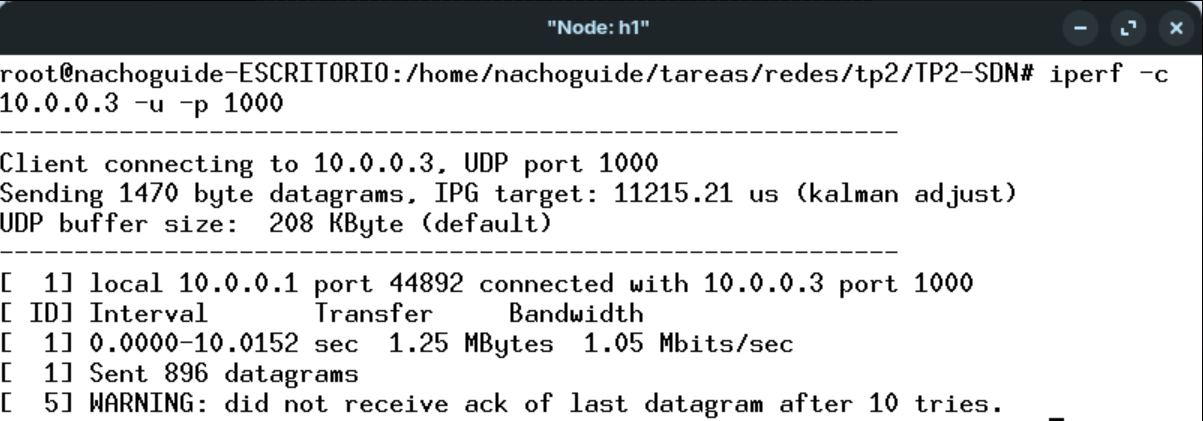
\includegraphics[width=0.7\textwidth]{img/regla3_h1_udp.png}
    \caption{Regla 3 desde el host 1 (UDP)}
\end{figure}

\begin{figure}[H]
    \centering
    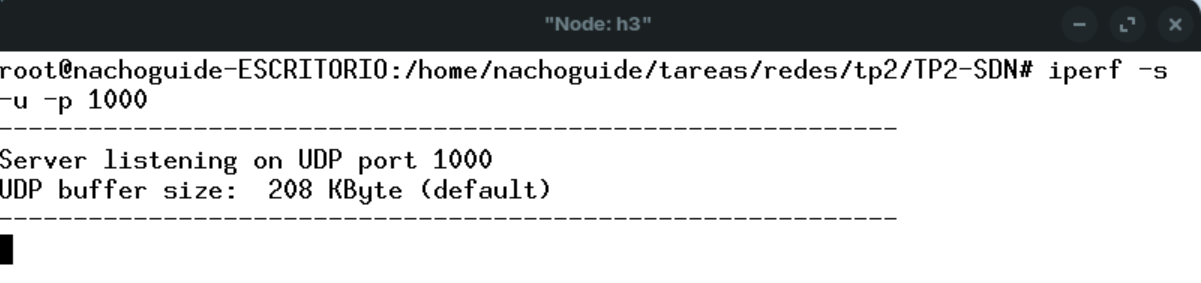
\includegraphics[width=0.7\textwidth]{img/regla3_h3_udp.png}
    \caption{Regla 3 desde el host 3 (UDP)}
\end{figure}

\begin{figure}[H]
    \centering
    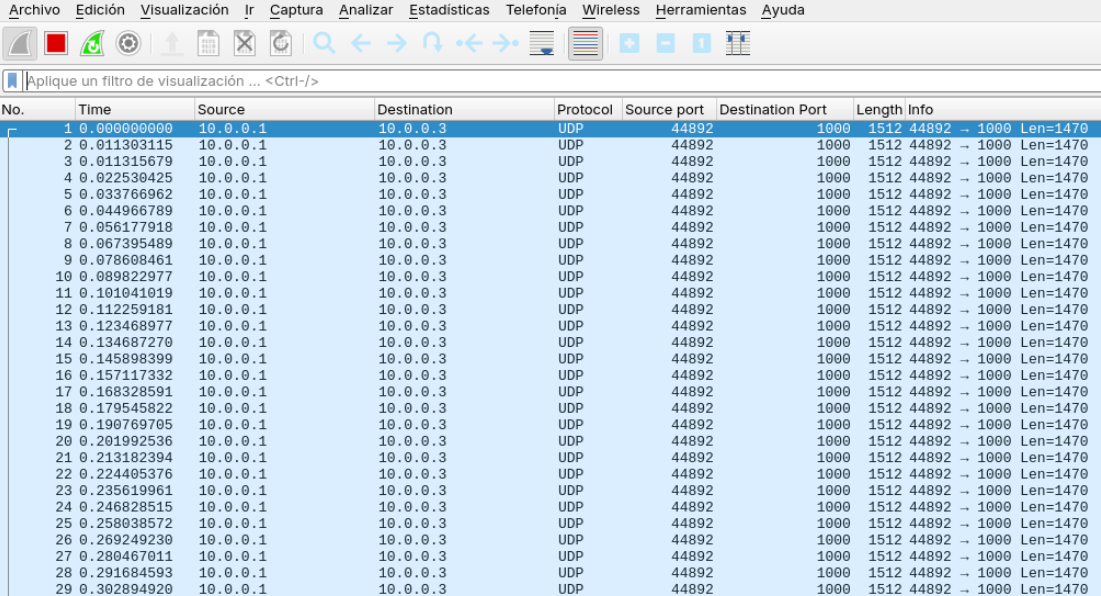
\includegraphics[width=0.7\textwidth]{img/regla3_wireshark_udp.png}
    \caption{Wireshark para la regla 3 (UDP)}
\end{figure}

Como resultado de esta prueba, el host 1 envió mensajes al host 3, pero no le llego respuestas por parte del host 3.


\section{Preguntas}\label{sec:preguntasAResponder}

    \subsection{¿Cuál es la diferencia entre un Switch y un router? ¿Qué tienen en común?}

    La diferencia principal entre un Switch y un Router radica en la capa del modelo de red en la que operan y el tipo de dirección que utilizan para reenviar los datos. Un Switch opera principalmente en la capa de enlace y utiliza direcciones MAC (direcciones de enlace) para el reenvío, mientras que un Router opera en la capa de red y sus decisiones de reenvío se basan en direcciones IP (direcciones de red). \\
    Tanto los switches como los routers comparten la función de conmutar paquetes, es decir, trasladar datos de un origen a un destino dentro de una red. Esta similitud funcional implica que ambos dispositivos deben enfrentar problemas similares, como la congestión de red.
    
    \subsection{¿Cuál es la diferencia entre un Switch convencional y un Switch OpenFlow?}

    ...
     
    \subsection{¿Se pueden reemplazar todos los routers de la Internet por switches OpenFlow? Piense en el escenario inter-ASes para elaborar su respuesta.}

    \begin{itemize}
        \item \textbf{Modelo de Control: Distribuido vs. Centralizado}
        \\ Una diferencia fundamental entre los routers convencionales y los switches OpenFlow radica en el modelo de control que utilizan. Los routers tradicionales operan bajo un esquema de control distribuido, donde cada dispositivo calcula de forma autónoma sus tablas de enrutamiento a través del intercambio de información con otros routers, usando protocolos como BGP. En contraste, los switches OpenFlow implementan un modelo de control lógicamente centralizado, en el que un controlador remoto —que posee una visión global del estado de la red— es responsable de calcular, instalar y actualizar las tablas de flujo de los switches. Esta arquitectura centralizada permite una programación más flexible y coordinada del comportamiento de la red, en comparación con la toma de decisiones local de los routers convencionales. \\
        
        \item \textbf{Escalabilidad y Autonomía en el Enrutamiento Inter-AS}

        Internet se estructura en miles de Sistemas Autónomos (AS), como los de un ISP o una gran organización. Esta organización responde principalmente a dos necesidades clave, la escalabilidad y la autonomía administrativa. A nivel de escalabilidad, sería inviable que cada router conociera todas las rutas posibles en Internet o difundiera constantemente información de estado a todos los demás dispositivos. Por otro lado, la autonomía permite que cada AS utilice sus propios algoritmos de enrutamiento interno y oculte detalles sobre su infraestructura.

        \item \textbf{Desafíos de SDN en el Entorno Inter-AS Global}

        Aunque las tecnologías como SDN y OpenFlow permiten que las redes sean más flexibles y fáciles de programar, su uso a gran escala (como en todo Internet) presenta grandes desafíos. Para reemplazar todos los routers actuales por switches OpenFlow, sería necesario un sistema de control central o varios controladores que trabajen en perfecta coordinación entre sí. Esto es muy difícil de lograr, ya que Internet está formado por miles de redes independientes (como los distintos ISP) que no siempre comparten información, objetivos o niveles de seguridad.
        
        
    \end{itemize}
    
    \section{Dificultades encontradas}\label{sec:dificultadesEncontras}
    Algunas dificultades que surgieron en el avance del proyecto fueron:
    
    \begin{itemize}
        \item ...
    \end{itemize}
    
\section{Conclusion}\label{conclusion}
    ...
    
\end{document}